\documentclass[12pt]{article}

\usepackage[T1]{fontenc}
\usepackage[utf8]{inputenc}
\usepackage{newtxtext,newtxmath}
\usepackage[margin=1in]{geometry}
\usepackage{graphicx}
\usepackage[section]{placeins}
\usepackage{subcaption}
\usepackage{booktabs}
\usepackage{array}
\usepackage{amsmath}
\usepackage{siunitx}
\usepackage{setspace}
\usepackage{parskip}
\usepackage[mathlines]{lineno}
\usepackage[font=small,labelfont=bf]{caption}
\usepackage{xurl}
\usepackage[hidelinks]{hyperref}
\usepackage[numbers,sort&compress]{natbib}

\graphicspath{{figures/}}
\setstretch{1.15}
\emergencystretch=2em
\widowpenalty=10000
\clubpenalty=10000
\renewcommand{\topfraction}{0.9}
\renewcommand{\bottomfraction}{0.8}
\renewcommand{\textfraction}{0.1}
\renewcommand{\floatpagefraction}{0.65}
\sisetup{detect-all}

\title{Machine-learning interatomic potentials for battery materials: Defect-dependent lithium adsorption and local transferability on graphene}

\author{Yuhan Sun$^{a,\dagger}$ and Xiao Huang$^{b,*,\dagger}$}
\date{}

\begin{document}
\linenumbers

\maketitle
\begin{center}
    \textit{$^{a}$University of Waterloo, Waterloo, ON N2L 3G1, Canada;\\
    $^{b}$Department of Chemistry, Duke University, Durham, NC 27708, USA}\\
    $^*$Corresponding author: Xiao Huang (Xiao.huang@duke.edu)\\
    $^\dagger$These authors contributed equally to this work.
\end{center}

\begin{abstract}
\linelabel{r2:abstract-start}
Defects in graphene change lithium adsorption, but their effect on the accuracy
of machine-learned interatomic potentials (MLIPs) is less clear. We use
spin-polarized density functional theory (DFT) and fine-tuned Message Passing
Atomic Cluster Expansion (MACE) models to examine pristine, monovacancy,
divacancy, and Stone--Wales graphene and a local Si$_4$--graphene motif.
PBE-D3(BJ) single-point calculations with a slab dipole correction give
fixed-geometry adsorption energies between -2.967 and -0.875 eV per Li.
Each of the sampled defect and Si-containing placements binds Li more strongly
than the sampled pristine placements; the monovacancy gives the strongest
binding. On independently selected perturbations around the five relaxed
structures, fine-tuning reduces the pooled force root-mean-square error from
450.0 to 267.5 meV \AA$^{-1}$ and improves accuracy in every structural family.
This improvement becomes smaller as the perturbation amplitude increases.
DFT tests of selected molecular-dynamics snapshots reveal a further dependence
on local chemistry: fine-tuning reduces the Si$_4$--graphene force error from
310 to 113 meV \AA$^{-1}$, while the monovacancy error remains near
1.1 eV \AA$^{-1}$. The latter snapshots contain unusually short C--C contacts
near the reconstructed vacancy. These results connect stronger Li adsorption
at defects with a need to test the potential on the specific local structures
it samples. Strained carbon configurations near monovacancies are a priority
for extending the present training set.\linelabel{r2:abstract-end}
\end{abstract}

\begin{flushleft}
\textbf{Keywords:} machine-learning interatomic potentials; MACE; artificial intelligence; battery materials; lithium adsorption; graphene defects
\end{flushleft}

\section{Introduction}

Defects in graphitic carbon create chemically distinct adsorption environments
for Li and can substantially change local binding relative to pristine graphene
\citep{uthaisar2010edge,zhou2012graphene,yildirim2014defect}. Vacancies expose
under-coordinated carbon atoms and permit local reconstruction, whereas a
Stone--Wales defect changes ring topology without removing carbon. Silicon adds
a different bonding environment and is widely studied in composite anodes,
although realistic Si-containing electrodes also involve alloying, volume
change, and heterogeneous microstructure \citep{obrovac2014alloy,sehrawat2021silicongraphene,palumbo2019siliconflg}.
Comparing these local environments at the dilute single-Li level provides a
controlled way to isolate how defect chemistry changes adsorption.

MLIPs can extend first-principles models toward larger configuration spaces and
finite-temperature sampling \citep{jacobs2025mlipguide}. MACE represents
higher-order atomic correlations through equivariant message passing
\citep{batatia2022mace}, and the MACE-MPA-0 foundation model provides a broad
starting point for materials chemistry \citep{batatia2025foundation}. Fine-tuning
can improve accuracy in a target domain \citep{radova2025finetuning}, but average
errors on configurations similar to the training data do not establish
reliability after defect reconstruction or large atomic displacement. Recent
studies have shown that training-set composition, foundation-model bias, and
potential-energy-surface softening can produce chemically specific
extrapolation failures \citep{niblett2025transferability,wong2026bias,deng2025softening}.

\linelabel{r2:concurrent-start}MLIP development commonly alternates sampling with new DFT calculations.
DeePMD-kit and the
DP-GEN concurrent-learning framework, for example, combine model training,
configuration-space exploration, ensemble-based model-deviation screening,
first-principles labeling, and iterative retraining
\citep{wang2018deepmd,zhang2020dpgen}. The present study uses
finite-temperature sampling and seed-resolved model comparisons, but it neither
applies a numerical model-deviation threshold nor performs a subsequent
retraining iteration. Direct DFT calculations instead establish the adsorption
trends and the range over which MLIP force predictions are supported, thereby
identifying local environments that require additional training data.\linelabel{r2:concurrent-end}

For defective graphene, an average error across several structures may conceal
poor predictions near one type of defect. Li adsorption energies describe the
relative stability of the sampled placements, whereas force comparisons test
whether the potential describes displaced atoms in those environments. Both
comparisons are needed to assess a model intended for finite-temperature sampling.

Here we address this question for pristine, monovacancy, divacancy, and
Stone--Wales graphene and a minimal Si$_4$--graphene motif. We establish
PBE-D3(BJ) adsorption-energy references with a slab dipole correction and test site
sensitivity across three PBE-ranked Li placements per family. We then compare
the MACE-MPA-0 foundation model with target-domain fine-tuning against an
independently defined DFT force benchmark spanning all five families and
against selected high-displacement monovacancy and Si$_4$--graphene snapshots.
The combination allows us to identify which local structures benefit from
fine-tuning and which require additional DFT training configurations.

\section{Computational methods}

\subsection{Model systems}

Five model systems were constructed with the Atomic Simulation Environment (ASE) \citep{larsen2017ase}: pristine graphene, monovacancy graphene, divacancy graphene, Stone--Wales graphene, and a Si$_4$--graphene motif. A graphene lattice parameter of 2.46 \AA{} and a 5 $\times$ 5 supercell gave an intact C$_{50}$ sheet. The 30.0 \AA{} cell height places 15.0 \AA{} of vacuum on each side of the initial graphene plane. A monovacancy was generated by removing one central C atom, and a divacancy was generated by removing a nearest-neighbor C--C pair. The Stone--Wales starting geometry was generated by rotating a central C--C bond. The resulting initial formulas were C$_{50}$Li, C$_{49}$Li, C$_{48}$Li, C$_{50}$Li, and C$_{50}$LiSi$_4$, respectively.

The Si-containing system places four non-substitutional Si atoms above the intact C$_{50}$ sheet and is described as a Si$_4$--graphene motif, not as a general Si--graphene composite. This motif is a deliberately minimal local model: four Si atoms are sufficient to introduce Si--Si bonding and local Li--Si/Si--C interactions without attempting to represent the alloying, volume expansion, and heterogeneous microstructure of realistic Si--graphene anodes \citep{obrovac2014alloy,sehrawat2021silicongraphene}. Its stability is therefore a DFT relaxation and adsorption question rather than an assumption built into the model. A Li atom was placed near the central adsorption region of each structure. Figure~\ref{fig:structures} defines the model families.

\begin{figure}[!t]
  \centering
  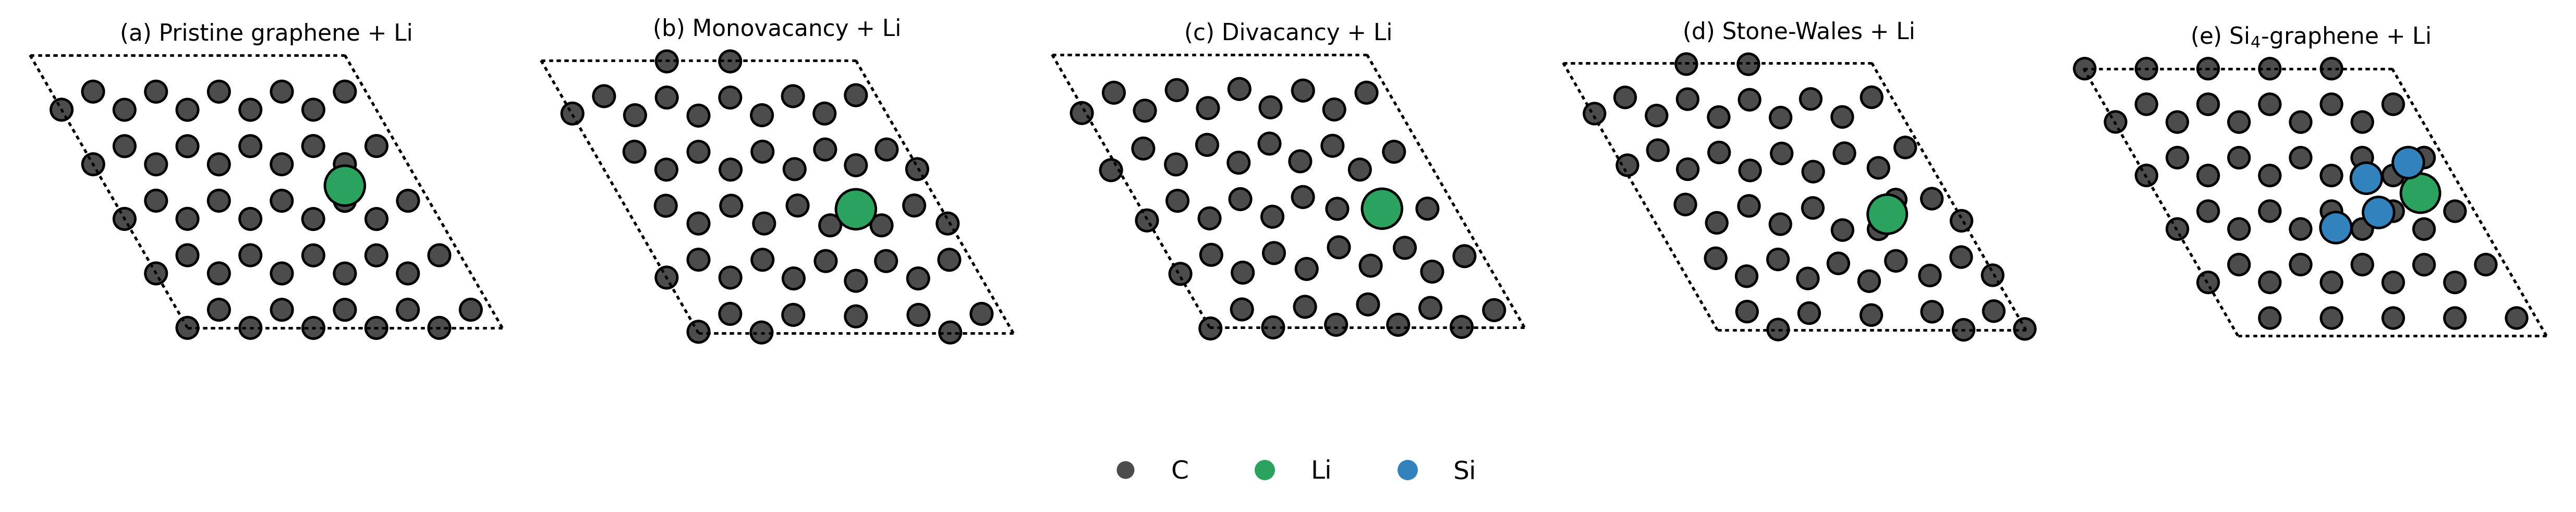
\includegraphics[width=\textwidth]{figures/structure_models.png}
  \caption{DFT-relaxed local structure families used for MACE labeling and analysis: pristine graphene, monovacancy graphene, divacancy graphene, Stone--Wales graphene, and a Si$_4$--graphene motif. Carbon, lithium, and silicon atoms are shown in gray, green, and blue, respectively. The final maximum force norm is below 0.02 eV \AA$^{-1}$ in every panel.}
  \label{fig:structures}
\end{figure}

\subsection{DFT labeling}

DFT calculations were performed with VASP 5.4.1 \citep{kresse1996efficient,kresse1996cms} using PAW potentials \citep{blochl1994paw,kresse1999paw} and the PBE exchange--correlation functional \citep{perdew1996pbe}. The PAW\_PBE datasets were C (08Apr2002), Li\_sv (10Sep2004), and Si (05Jan2001). The calculations used spin polarization, ENCUT = 520 eV, a Gamma-centered 3 $\times$ 3 $\times$ 1 k-point mesh, Gaussian smearing with ISMEAR = 0 and SIGMA = 0.05 eV, PREC = Accurate, LREAL = Auto, ALGO = Normal, NELM = 120, LASPH = .TRUE., ADDGRID = .TRUE., and ISYM = 0. Initial magnetic moments were 0.1 $\mu_{\mathrm B}$ on C and Si and 1.0 $\mu_{\mathrm B}$ on Li. The final total moments of the relaxed pristine, monovacancy, divacancy, Stone--Wales, and Si$_4$--graphene structures were 0.000, 0.814, 0.000, 0.300, and 0.561 $\mu_{\mathrm B}$, respectively. All ionic coordinates were relaxed without selective-dynamics constraints at fixed lattice vectors using IBRION = 2, ISIF = 2, NSW = 100, EDIFF = $10^{-5}$ eV, and EDIFFG = -0.02 eV \AA$^{-1}$. The final maximum atomic force norms span 0.0183--0.0193 eV \AA$^{-1}$ across the five relaxed structures. Single-point site and path-scan labels used IBRION = -1, NSW = 0, and EDIFF = $10^{-6}$ eV. The MACE training labels did not include an explicit vdW correction or slab dipole correction. This omission is important because Li adsorption on graphitic surfaces and one-sided slab adsorbates can be sensitive to both effects \citep{grimme2010d3}.

Additional adsorption calculations therefore used fixed-geometry single points on
the current Li+substrate and Li-removed substrate geometries with IBRION = -1,
NSW = 0, EDIFF = $10^{-6}$ eV, LREAL = .FALSE., and the same
3 $\times$ 3 $\times$ 1 slab k-point mesh. Each slab calculation used a
two-stage electronic protocol. A PBE-D3(BJ) preconditioning stage (IVDW = 12)
used ALGO = Normal, NELM = 180, and no dipole correction. The converged
wavefunctions and charge density were then restarted with ALGO = All,
TIME = 0.4, NELM = 240, and the slab dipole correction
(LDIPOL = .TRUE., IDIPOL = 3). Electronic convergence of the final PBE-D3(BJ)
calculation required normal termination and a final electronic iteration below NELM
\citep{grimme2010d3,grimme2011bj}. A separate isolated Li atom reference used
a 20 \AA{} cubic cell, a Gamma-only 1 $\times$ 1 $\times$ 1 mesh, and
EDIFF = $10^{-7}$ eV. Adsorption energies are reported as
\linelabel{r2:ads-eq-start}
\begin{linenomath}
\begin{equation}
  E_{\mathrm{ads}} = E(\mathrm{Li+substrate}) - E(\mathrm{substrate}) - n_{\mathrm{Li}}E(\mathrm{Li\ atom}).
\end{equation}
\end{linenomath}
These calculations provide adsorption-energy references for the current geometries, not exhaustive relaxed adsorption-site searches.\linelabel{r2:ads-eq-end}

Site sensitivity was examined without changing this thermodynamic scope. For
each family, the three lowest-energy placements from the preceding PBE
fixed-geometry site scan were selected before the new calculations and
re-evaluated with the same PBE-D3(BJ), dipole-corrected single-point protocol.
The substrate coordinates are identical among the selected placements within a
family, so one common substrate reference is used for their adsorption energies.
These calculations test whether the family comparison is tied to one Li
placement; they remain fixed-geometry comparisons rather than relaxed adsorption-site
searches.

The final MACE dataset contains 273 frames: 194 frames from ionic relaxation trajectories and 79 fixed-geometry site/path single-point calculations. Site labels sample the initial Li position, hollow-like sites, bridge-like sites, top-like sites, and Si$_4$-related positions. Path labels are linear Cartesian interpolation images between two sampled endpoints. This deliberately compact dataset samples five local chemical families and selected displacement coordinates; it is not intended to exhaust the configurational space of defective graphene or Si-containing electrodes. Direct DFT force comparisons on displaced configurations therefore provide the transferability test rather than the dataset size alone. The path quantities below are fixed-geometry path-scan descriptors and endpoint energy differences, not climbing-image NEB results or migration barriers \citep{henkelman2000neb}.

All 273 DFT labels satisfy the electronic-convergence criterion, with the final
electronic iteration below \texttt{NELM}. Frame-level convergence records are
provided in the Supplementary Data.

Figure~\ref{fig:si_dataset_counts} shows the number of configurations in each
family. Relaxation frames sample neighboring geometries along optimization
trajectories, while the site and path calculations vary the Li position with
the substrate fixed. These sources provide complementary local coverage but
also introduce correlations that must be considered when splitting the data.

\begin{figure}[!htbp]
  \centering
  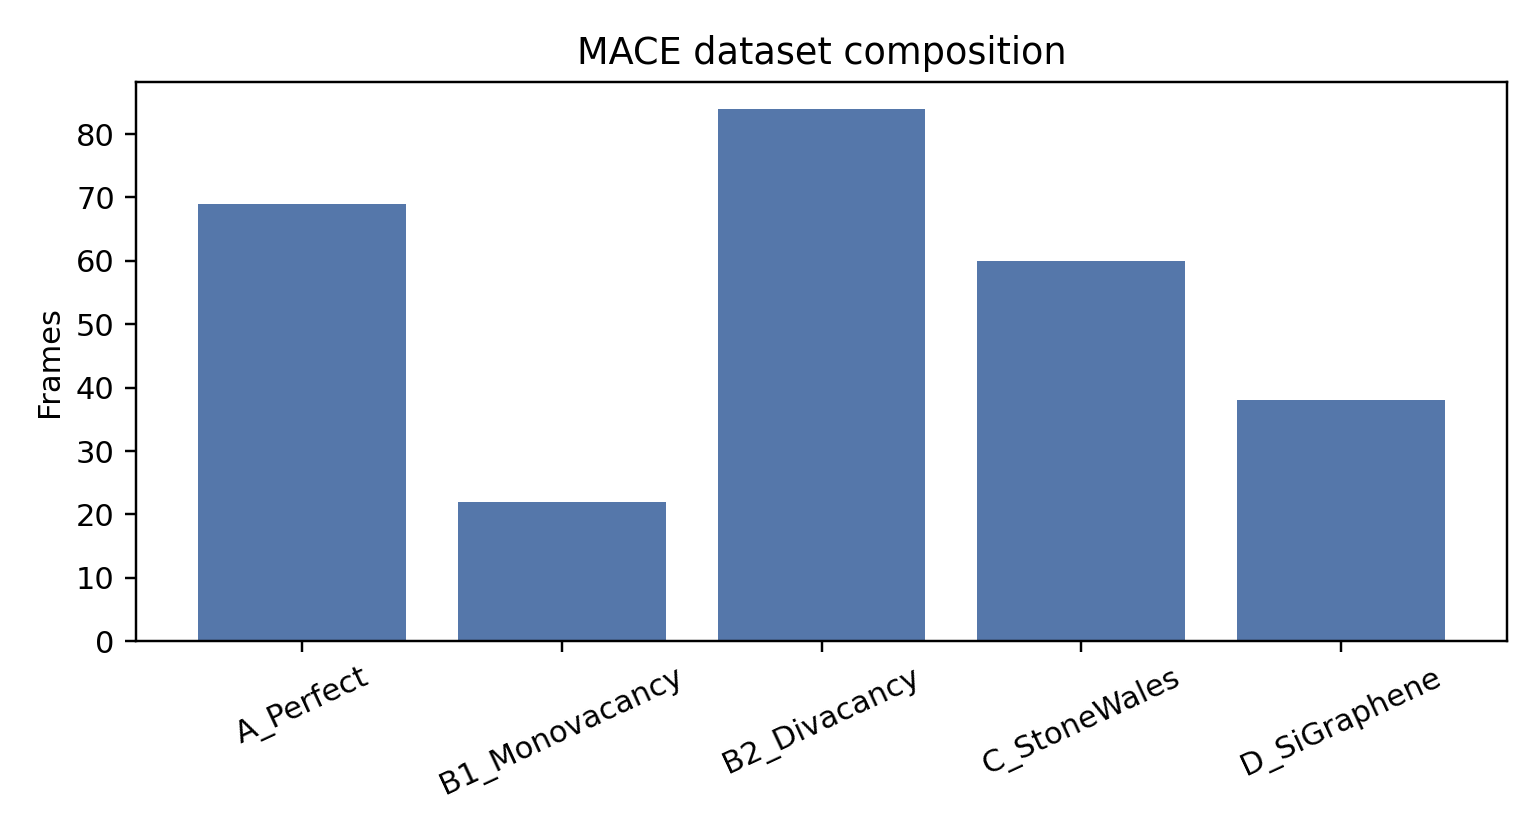
\includegraphics[width=0.72\textwidth]{dataset_family_counts.png}
  \caption{Number of DFT-labeled configurations in each structural family.}
  \label{fig:si_dataset_counts}
\end{figure}


\subsection{Potential development workflow}

\linelabel{r2:workflow-start}The DFT-labeled structures were converted to extended XYZ files. An initial split contained 211 training frames, 31 validation frames, and 31 test frames, but correlated images from individual interpolation paths occurred in more than one partition. We therefore use this split only to characterize interpolation within the sampled configurations. For a correlation-controlled split, every relaxation trajectory remains in training, all images from a fixed path remain in one group, and the remaining site/path groups are sorted within each structural family and assigned by a deterministic 8:1:1 train/validation/test cycle. The resulting split contains 263 training frames, 5 validation frames, and 5 test frames, with one configuration from each family in both validation and test. Because these held-out sets are small, they assess sensitivity to cross-partition correlation rather than population-level transferability.

The MACE-MPA-0 medium foundation model \citep{batatia2025foundation} was fine-tuned from the checkpoint \path{mace-mpa-0-medium.model}. Its inherited architecture used a 6.0 \AA{} radial cutoff, two interaction layers, hidden irreducible representations \(128\times 0e + 128\times 1o\), correlation order 3, and spherical harmonics through \(l=3\). The architecture was retained without screening against the present test configurations. A reference model trained with MACE 0.3.15 and seed 20260427 was used for the original interpolation-error comparison and the 500 ps trajectories. Training used double precision, batch size 2, 300 epochs, an initial learning rate of \(5\times 10^{-4}\), Adam/AMSGrad optimization with weight decay \(5\times 10^{-7}\), exponential moving-average decay 0.99, and stochastic weight averaging from epoch 225. First-stage energy and force weights were 1.0 and 100.0; the second-stage weights were 1000.0 and 100.0.

The three-seed committee and grouped-$E_0$ models used MACE 0.3.16, batch size 4, 300 epochs, an initial learning rate of $10^{-3}$, and the same epoch-225 stochastic-weight-averaging transition. The committee models used single precision, whereas the grouped-$E_0$ model used double precision. Embedding and interaction blocks were frozen, while product and readout blocks remained trainable. Epochs 224 and 298 were used for first- and second-stage evaluation, respectively, according to the validation metric. To correct the large Si$_4$--graphene energy offset in the initial model, foundation-assisted $E_0$ estimation was performed over all 263 grouped training configurations. The deterministic linear solve had full elemental rank (3/3) and produced baseline offsets of -3.271318, -1.246324, and -1.280346 eV for Li, C, and Si, respectively. Acceptance required finite coefficients and full elemental rank; there was no iterative convergence threshold for this solve. These quantities are model energy offsets rather than isolated-atom energies. Complete training commands and model records are provided in the Supplementary Data.

We report the original correlated-split errors as an interpolation baseline and use
the grouped split and corrected $E_0$ model for the high-displacement force
comparison. A direct comparison with the unfine-tuned MACE-MPA-0 foundation
model determines whether target-domain fine-tuning improves each selected local
environment. Three additional random-seed models quantify training sensitivity;
their validation metrics are reported in Section~\ref{sec:interpolation}. The
three-member committee is used only as a qualitative seed-sensitivity diagnostic.
No numerical committee-disagreement or force-deviation threshold is used to
select configurations for DFT, so it should not be interpreted as a calibrated
uncertainty ensemble of the type used in concurrent-learning workflows.

\linelabel{r2:committee-start}Table~\ref{tab:si_concurrent_learning} summarizes the relationship to DP-GEN.
The DFT-labeled MD snapshots are retained as test configurations in this study;
incorporating them into training would require a new independent test set.\linelabel{r2:committee-end}

\begin{table}[!htbp]
  \centering
  \small
  \caption{Relationship between a representative concurrent-learning workflow
  and the validation-driven procedure used here.}
  \label{tab:si_concurrent_learning}
  \setlength{\tabcolsep}{4pt}
  \begin{tabular}{>{\raggedright\arraybackslash}p{2.0cm}>{\raggedright\arraybackslash}p{5.0cm}>{\raggedright\arraybackslash}p{7.1cm}}
    \toprule
    Aspect & DP-GEN concurrent learning & Present study \\
    \midrule
    Potential model & Deep Potential ensemble & Fine-tuned MACE-MPA-0 models \\
    Exploration & Iterative configuration-space sampling & Finite-temperature
    trajectories used to generate displaced test configurations \\
    Selection signal & Quantitative ensemble model deviation & High displacement
    and qualitative seed sensitivity; no calibrated deviation threshold \\
    First-principles step & Labels selected uncertain configurations & Tests MACE
    forces and identifies chemistry-specific failure modes \\
    Retraining loop & Selected labels are added and the cycle is repeated & The DFT
    snapshots are not added to a subsequent training cycle \\
    Primary purpose & Expand the range described by the potential & Determine
    which adsorption and force predictions are supported by DFT \\
    \bottomrule
  \end{tabular}
\end{table}


An additional force benchmark was defined after model training without using
predicted energies, forces, or committee disagreement for configuration
selection. Starting from the converged DFT geometry of each family, five
deterministic Cartesian perturbations were generated with per-coordinate
Gaussian standard deviations of 0.03, 0.06, 0.06, 0.10, and 0.10 \AA{}.
The mean displacement was removed from each configuration, and deterministic
resampling rejected any geometry with a minimum interatomic distance below
1.15 \AA{}. The resulting balanced set contains 25 configurations, five per
family. Spin-polarized PBE single points used the 520 eV cutoff, the
3 $\times$ 3 $\times$ 1 mesh,
\texttt{LREAL = .FALSE.}, and an electronic threshold of $10^{-6}$ eV. This
predefined set tests local force robustness around all five converged
structures. Because the perturbations originate from those structures, it is
not treated as exhaustive configurational or dynamical validation. All 25 DFT
calculations converged electronically with final iterations below
\texttt{NELM} and yielded finite energies and forces.\linelabel{r2:workflow-end}

For each configuration, the force RMSE is the square root of the mean squared
MACE--DFT difference over all Cartesian force components. The balanced benchmark
pools those components across configurations. The correlated-split and MD
snapshot summaries instead take the root mean square of the configuration-level
RMSEs, giving each configuration equal weight. The two definitions coincide
within a family of fixed atom count but can differ when families are combined.

\subsection{Finite-temperature snapshot generation}

LAMMPS (10 September 2025) \citep{plimpton1995lammps} simulations used the
converted MACE models with the MACE pair style. The five structures were
replicated 2 $\times$ 2 $\times$ 1, giving 196--220 atoms and four Li atoms per
cell, equivalent to one Li per original 5 $\times$ 5 graphene supercell or an
areal density of $7.63\times10^{13}$ cm$^{-2}$. The systems were sampled at
400 K with a 1 fs timestep after 10 ps of Nos\'e--Hoover NVT equilibration; the
thermostat damping time was 0.1 ps. These
finite-temperature trajectories were used to generate displaced configurations,
not to determine diffusion coefficients. Their physical reliability was assessed
through direct DFT force comparisons rather than trajectory stability alone.
Nine selected high-displacement snapshots
(three monovacancy and six Si$_4$--graphene) were evaluated directly with
spin-polarized DFT and Gamma-only sampling. Five final outputs used
ALGO = Normal, EDIFF = $10^{-6}$ eV, and NELM = 160; four final outputs used a
two-stage ALGO = All calculation with TIME = 0.2: an EDIFF = $10^{-4}$ eV,
NELM = 180 preconditioning stage followed by a restart at
EDIFF = $10^{-6}$ eV and NELM = 240. All nine calculations used in the force
comparison converged electronically and yielded finite forces. Frame-level force
RMSE was computed against both MACE-MPA-0 and the
grouped-$E_0$ fine-tuned model. Seven additional Si$_4$--graphene snapshots from
longer trajectories received converged DFT single-point calculations. In total, 16
electronically converged DFT snapshot calculations are summarized
in Tables~\ref{tab:si_initial_snapshots} and \ref{tab:si_extended_snapshots}.
Only the initial nine are included in the force-error comparison. None of these DFT-validated snapshots is
incorporated into a subsequent MACE training cycle in the present work. They
define targets for a future dataset-expansion and retraining iteration; a closed
active-learning cycle is beyond the scope of this study.

\linelabel{r2:msd-eq-start}After equilibration, the LAMMPS \texttt{compute msd} calculation was reset for
the four Li atoms with \texttt{com yes}. The in-plane displacement is
\begin{linenomath}
\begin{equation}
 M_{xy}(t)=\frac{1}{N_{\mathrm{Li}}}\sum_{i=1}^{N_{\mathrm{Li}}}
 \left\lVert \Delta\mathbf r_{i,xy}(t)
 -\frac{1}{N_{\mathrm{Li}}}\sum_{j=1}^{N_{\mathrm{Li}}}
 \Delta\mathbf r_{j,xy}(t)\right\rVert^2,
 \label{eq:msd}
\end{equation}
\end{linenomath}
where $N_{\mathrm{Li}}=4$ and each displacement is calculated from unwrapped
coordinates relative to the start of production. Removing Li-group
center-of-mass motion makes this a measure of relative spreading of the four
Li atoms. We use it to describe the configurations sampled over a finite time
window and do not extract a diffusion coefficient.\linelabel{r2:msd-eq-end}

\section{Results and Discussion}

\subsection{Defect-dependent Li adsorption}

The five structures create a wide range of local Li binding strengths
(Fig.~\ref{fig:scientific_summary}a). The PBE-D3(BJ) fixed-geometry adsorption
energy is -0.634 eV per Li for pristine graphene. Relative to this reference,
the monovacancy and Si$_4$--graphene geometries are more favorable by 2.481 and
2.715 eV, respectively, and the divacancy is more favorable by 0.694 eV. The
sampled Stone--Wales geometry instead gives a slightly positive adsorption
energy of +0.009 eV, 0.643 eV less favorable than pristine graphene.

The strong monovacancy value is consistent with the chemically intuitive role
of under-coordinated and reconstructed carbon near a vacancy, while the Si$_4$
motif introduces direct Li--Si and Si--C environments absent from pristine
graphene. The divacancy produces an intermediate response, showing that the
removal of carbon atoms alone does not determine the adsorption strength; the
result depends on the resulting local topology. The Stone--Wales result likewise
shows that a topological defect need not strengthen Li binding for the sampled
geometry. Complete fixed-site rankings are provided in the Supporting
Information.

\begin{figure}[!t]
  \centering
  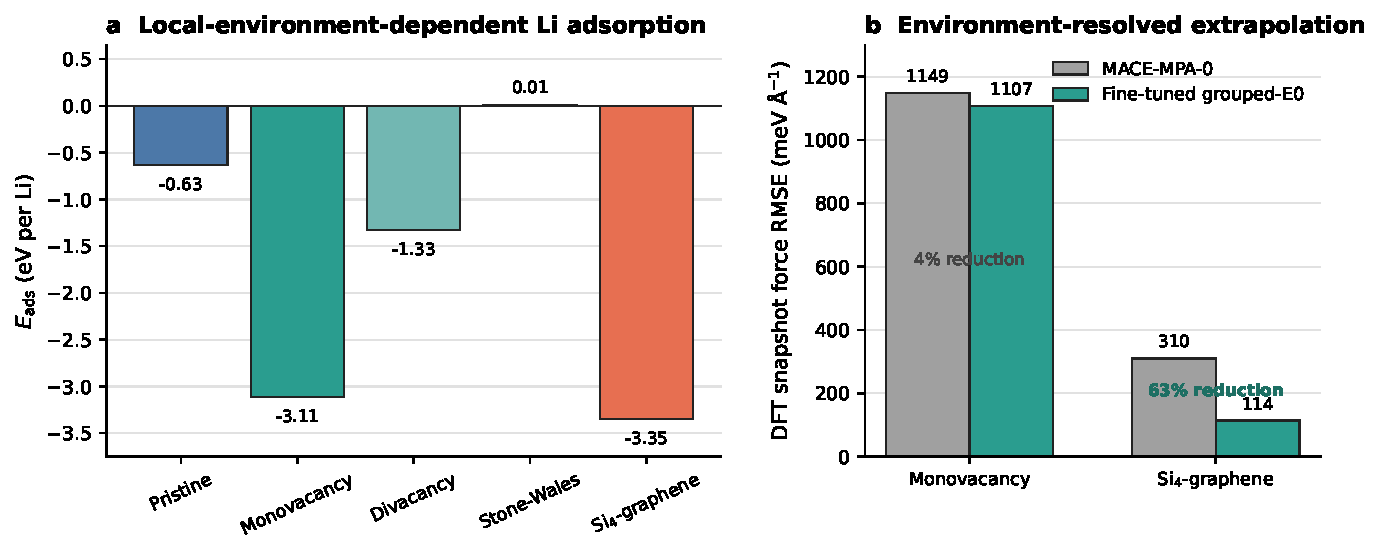
\includegraphics[width=\textwidth]{figures/scientific_summary_reframe.pdf}
  \caption{Local-environment dependence of Li adsorption and MLIP
  transferability. (a) PBE-D3(BJ) fixed-geometry adsorption energies with a slab
  dipole correction. More negative values indicate stronger adsorption relative
  to an isolated Li atom. (b) Frame-level force RMSE against DFT for selected
  high-displacement monovacancy (three frames) and Si$_4$--graphene (six frames)
  snapshots. Fine-tuning strongly improves the Si$_4$ subset but leaves the
  monovacancy subset near 1.1 eV \AA$^{-1}$.}
  \label{fig:scientific_summary}
\end{figure}

These adsorption energies compare one current geometry per family and therefore
establish local energetic anchors rather than fully optimized adsorption
thermodynamics. In particular, they do not include an exhaustive relaxed-site
search, Li--Li clustering, multilayer graphite, or electrode--electrolyte
effects. Within this defined single-geometry comparison, however, the 3.358 eV
span directly demonstrates that the five local environments probe substantially
different Li chemistry.

\subsection{Fine-tuning improves interpolation within the sampled workflow}

The 273-frame DFT label set spans all five structural families. On the original
same-workflow test split, the MACE-MPA-0 foundation model gives an all-family
force RMSE of 285.2 meV \AA$^{-1}$, whereas the first fine-tuned model gives
20.1 meV \AA$^{-1}$. Thus, target-domain fine-tuning reduces the force error by
92.9\% for configurations drawn from the same relaxation and site/path sampling
workflow.

This comparison establishes a real interpolation improvement, but it is not the
transferability test used for the central conclusion. Images from the same fixed
interpolation paths were correlated across the original train, validation, and
test partitions. We therefore rebuilt the data split by keeping each path group
intact and corrected the elemental energy baseline through foundation-assisted
$E_0$ estimation. The resulting grouped test set contains one configuration per
family and is too small for population-level error estimates. Full split
definitions, family-resolved same-workflow errors, $E_0$ fitting details, and
three-seed sensitivity results are reported in the Supporting Information. The
scientifically more demanding comparison is the direct DFT test on displaced
configurations described next.

\subsection{Transferability is local-environment dependent}

The nine selected finite-temperature snapshots provide an explicit test outside
the small-displacement labeling workflow (Fig.~\ref{fig:scientific_summary}b).
For the unfine-tuned foundation model, the frame-level force RMSE is
1149 meV \AA$^{-1}$ for the three monovacancy snapshots and
310 meV \AA$^{-1}$ for the six Si$_4$--graphene snapshots. The grouped-$E_0$
fine-tuned model reduces the Si$_4$ error to 114 meV \AA$^{-1}$, a 63\%
improvement, but changes the monovacancy error only to
1107 meV \AA$^{-1}$, a 4\% improvement. Across all nine frames, the corresponding
RMSE changes from 710 to 646 meV \AA$^{-1}$.

This contrast is the central transferability result. Fine-tuning is effective
for the selected Si-containing configurations but does not supply the force
physics required for the reconstructed monovacancy configurations. The
monovacancy snapshots contain minimum C--C distances of 1.204--1.217 \AA{}, much
shorter than an equilibrium graphitic C--C bond, whereas the selected Si$_4$
snapshots retain minimum C--C distances near 1.36 \AA{} and include Si--Si
contacts down to 1.994 \AA{}. The large monovacancy force errors therefore align
with a specific structural regime: highly strained local carbon reconstruction.
They are not explained by a uniform loss of accuracy across all displaced
configurations.

Aggregate interpolation metrics would obscure this difference. The
same-workflow 20.1 meV \AA$^{-1}$ force RMSE is more than an order of magnitude
smaller than either high-displacement family error, yet the two families respond
very differently to corrected fine-tuning. For active learning, the appropriate
next data are therefore not additional near-equilibrium frames sampled in the
same proportions. They are DFT configurations that resolve strained C--C
reconstruction and Li coordination near monovacancies, together with
family-balanced displaced configurations that test whether the observed
contrast persists beyond the present nine frames. The present DFT-validated
snapshots identify that next sampling target but have not been incorporated into
a further training cycle; the work therefore does not constitute a closed
concurrent-learning loop.

\subsection{Scope and limitations}

The present evidence supports two linked conclusions: local defect chemistry
changes dilute Li adsorption, and local environment also controls the
extrapolative reliability of the fine-tuned MLIP. The numerical adsorption
values remain fixed-geometry single-point anchors, and the environment-resolved
force comparison contains three monovacancy and six Si$_4$ frames. The
Si$_4$--graphene structure is a minimal local motif rather than a representative
composite anode. Fixed interpolation paths and finite-window trajectories are
included in the Supporting Information as data-generation context; they are not
used to infer migration barriers or diffusion coefficients. These boundaries do
not alter the observed contrast between the two snapshot subsets, but they set
the scale of the conclusions and motivate broader, family-balanced DFT sampling.



\section{Conclusion}

\linelabel{r2:conclusion-start}Defect chemistry changes both Li adsorption and MLIP reliability in the present
graphene-based environments. Across three evaluated placements per family,
all 12 non-pristine geometries bind Li more strongly than all three
pristine geometries. The best sampled adsorption energies are -0.918, -2.967,
-2.301, -1.587, and -2.465 eV per Li for pristine, monovacancy, divacancy,
Stone--Wales, and Si$_4$--graphene, respectively, and the preceding PBE site
order is retained in every family. On the predefined 25-configuration force
benchmark, target-domain MACE fine-tuning lowers pooled force RMSE from 450.0
to 267.5 meV \AA$^{-1}$ and lowers the family-resolved error in all five
environments. The benefit is not uniform outside that local perturbation
regime: fine-tuning reduces the selected Si$_4$ high-displacement force RMSE
from 310 to 113 meV \AA$^{-1}$ but leaves the reconstructed-monovacancy error at
1097 meV \AA$^{-1}$.

The monovacancy binds Li most strongly among the sampled placements and also
produces the largest force errors in the selected MD snapshots. The improvement
on small perturbations does not extend to its highly strained carbon
configurations. Additional training should therefore include short C--C
contacts and Li coordination changes near monovacancies, followed by independent
tests across all five families. Relaxed adsorption-site searches and broader
snapshot sampling would extend the scope of the present fixed-geometry and
local-force comparisons.\linelabel{r2:conclusion-end}

\section*{Supplementary Data}

Supplementary Data contains the machine-readable configurations, force labels,
model checkpoints, numerical tables, and scripts needed to reproduce the
analyses. All scientific figures and summary tables are included in the main
article.

\section*{Data and Code Availability}

A version-pinned reproducibility archive is provided with this article as
Supplementary Data. It contains the code, manuscript source, curated figures,
input and validation scripts, the five author-trained model checkpoints, and
the compact submission data. The archive includes the 273-frame extxyz dataset,
original and group-held-out split definitions, numerical evidence tables, a
file-level SHA256 manifest, and a source-commit identifier in the ZIP metadata.
The curated scientific data are licensed under CC BY 4.0, and the analysis and
workflow code is licensed under MIT. Larger processed outputs and raw runtime
files are excluded; their scope is documented in the reproducibility manifest,
and they are available from the corresponding author on reasonable request.

Licensed VASP POTCAR files, WAVECAR/CHGCAR files, and full raw OUTCAR files are not redistributed. For traceability, evidence tables record input-generation scripts, convergence flags, parsed energies/forces, file sizes, modification times, and hashes.

\section*{Funding}

This research did not receive any specific grant from funding agencies in the public, commercial, or not-for-profit sectors.

\section*{Credit authorship contribution statement}

Yuhan Sun and Xiao Huang contributed equally to Conceptualization, Methodology,
Software, Validation, Formal analysis, Investigation, Data curation,
Visualization, Writing--original draft, and Writing--review and editing.
Xiao Huang additionally contributed Supervision.

\section*{Declaration of competing interests}

The authors declare that they have no known competing financial interests or personal relationships that could have appeared to influence the work reported in this paper.

\section*{Declaration of generative AI and AI-assisted technologies in the manuscript preparation process}

During the preparation of this work, the authors used OpenAI Codex to support language editing, consistency checks, and code-assisted verification of manuscript reported values. After using this tool, the authors reviewed and edited the content as needed and take full responsibility for the content of the published article.

\begingroup
\footnotesize
\setstretch{1.0}
\setlength{\bibsep}{0pt plus 0.3ex}
\bibliographystyle{achemso}
\bibliography{references}
\endgroup

\end{document}
